% Beamer slide template prepared by Tom Clark <tom.clark@op.ac.nz>
% Otago Polytechnic
% Dec 2012

\documentclass[10pt]{beamer}
\usetheme{Dunedin}
\usepackage{graphicx}
\usepackage{fancyvrb}

\newcommand\codeHighlight[1]{\textcolor[rgb]{1,0,0}{\textbf{#1}}}

\title{SOLID}

\author[IN608]{Intermediate Application Development}
\institute[Otago Polytechnic]{
  Otago Polytechnic \\
  Dunedin, New Zealand \\
  Kaiako: Tom Clark
}
\date{}
\begin{document}

%----------- titlepage ----------------------------------------------%
\begin{frame}[plain]
  \titlepage
\end{frame}

%----------- slide --------------------------------------------------%
\begin{frame}
  \frametitle{Background}
  
  In the 1990's (and earlier), software developers noted that a distressing number 
  of projects went badly or failed outright. Literature emerged examining reasons for this
  analysing why this was happening and what could be done to improve software development.
  
  Among other things, practioners sought to identify a set of good development practices and patterns.
  One very influential article was \emph{Design Principles and Design Patterns} by Robert C. Martin.
\end{frame}

%----------- slide --------------------------------------------------%
\begin{frame}
  \frametitle{Bit rot}
  
  Martin noted that problems arise when software changes, either during initial
  development or later in its life. He called these problems ``rot'' and he identified
  various types of this rot.
  
  \end{frame}

%----------- slide --------------------------------------------------%
\begin{frame}
  \frametitle{Bit rot}
  
  Martin noted that problems arise when software changes, either during initial
  development or later in its life. He called these problems ``rot'' and he identified
  various causes this rot.
  
  \end{frame}

%----------- slide --------------------------------------------------%
\begin{frame}
  \frametitle{Causes of rot}
  
  \begin{description}
    \item[Rigidity] Code that is difficult to change because changes to
    one part requires changes to many other parts
    \item[Fragility] Making a change at one point in the code causes it to
    break in other parts
    \item[Immobility]Modules can't be moved into other projects or places within a project even
    when the intended function is the same.
    \item[Viscosity]It's easier to make changes in a bad or hackish way than in a ``good'' way. 
  \end{description}
  
  Most of these problems step from overly tight coupling of modules, or badly structured dependencies.
  
  \end{frame}

%----------- slide --------------------------------------------------%
\begin{frame}
  \frametitle{SOILD}
  
  Martin went on to identify five design principles that help make code
  resistent to rot. These have come to be known as the SOILD principles.
  
    
\end{frame}

%----------- slide --------------------------------------------------%
\begin{frame}[fragile]
  \frametitle{Single Responsibility Principle}
  
  A class should have only one reason to change.
  
  Consider a class like this one:
  
  \begin{verbatim}
  class ReportGenerator
    read_data()
    calculate_results()
    write_report()
  \end{verbatim}
  
  We might change this class if
  \begin{enumerate}
    \item the data sources change,
    \item the formulas to calculate results change,  
    \item the report format changes.
  \end{enumerate}
  
  This code is immobile. If we need to use the \texttt{calculate\_results()} method in a different setting, this class isn't useful.  
  
  
    
\end{frame}

%----------- slide --------------------------------------------------%
\begin{frame}[fragile]
  \frametitle{Single Responsibility Principle}
  
  We can fix this by splitting this into three classes
  
  \begin{verbatim}
    class DataReader
    
    class ResultCalculator
    
    class ReportWriter
  \end{verbatim} 
    
\end{frame}

%----------- slide --------------------------------------------------%
\begin{frame}[fragile]
  \frametitle{Open-Closed Principle}
  
  A class should be open for extension but closed for modification.
  
  Consider a class like this:
  
  \begin{verbatim}
  
  class DataRecord  
  
      save_to_db()
        if db_type == MYSQL:
          # mysql-specific code
        else if db_type == POSTGRES:
          # postgres-specific code
        ...  
   \end{verbatim}
   
   Now suppose we want to add support for SQL Server.
   
   This code is viscous, and probably also rigid.         
  
\end{frame}  

%----------- slide --------------------------------------------------%
\begin{frame}
  \frametitle{Liskov Substitution Principle}
  
  Objects of a class should be replaceable by instances of subclasses.
  
  Suppose that we start our project using MySQL and build a MySQL interface class.
  
  \vspace{5mm}
  Later we decide to add support for Postgres, so we create a new class that inherits from 
  the original MySQL class since it has the same behaviours.  But there is never a case 
  where we ask for a MySQL object and will be happy getting a Postgres one instead.
  \end{frame} 
  
%----------- slide --------------------------------------------------%
\begin{frame}
  \frametitle{Liskov Substitution Principle}
  
  A better solution is to create a base \texttt{Database} class (probably abstract) and derive
  two child classes, one for MySQL and one for Postgres. 
  
  \vspace{5mm}
  In a situation where the specific DBMS doesn't matter, we can specify the base \texttt{Database}
  class. If we get either of the child classes, then this will work. Note that we also need to write the 
  child classes so that they satisfy the intent of the parent class.
  \end{frame} 

%----------- slide --------------------------------------------------%
\begin{frame}
  \frametitle{Interface Segregation Principle}
  
  A class should not depend on an interface it does not use.
  
  \vspace{5mm}
  
  Suppose we have a hierarchy of database interface classes.
  
  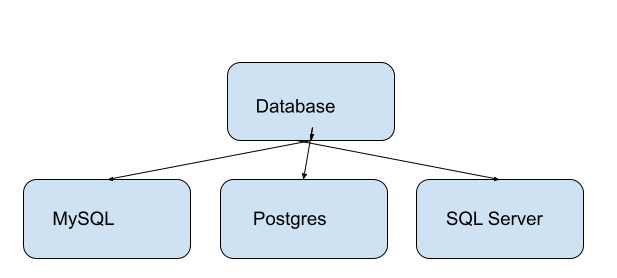
\includegraphics[width=5cm]{db1.png}
  
  Now let's add some new types of database systems.
  
  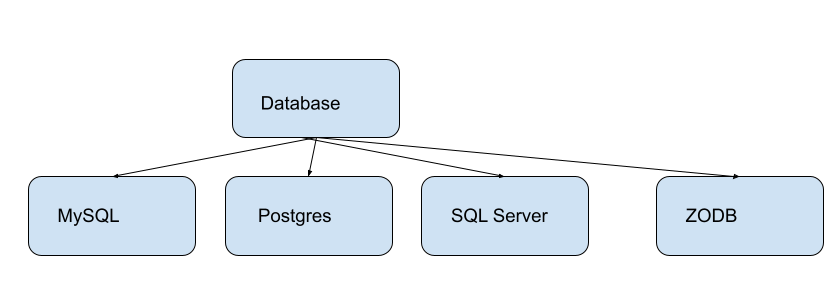
\includegraphics[width=6cm]{db2.png}
\end{frame}  
 
%----------- slide --------------------------------------------------% 
\begin{frame}
  \frametitle{Interface Segregation Principle}
  
  The problem is that ZODB is an object database, while the previous
  classes all worked with relational databases. The base class may contain 
  code that is specific to relational databases that ZODB does not use.
  
  \vspace{5mm}
  
    
  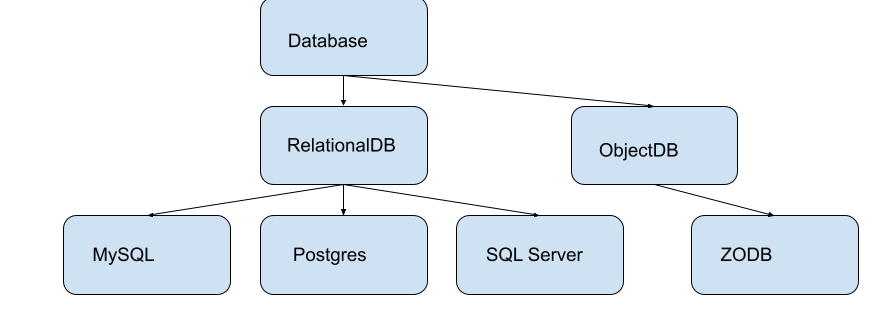
\includegraphics[width=6cm]{db3.png}
  
  \begin{itemize}
    \item Let \texttt{Database} define an interface common to all database systems.
    \item Let \texttt{RelationalDB} define the interface for relational databases.
    \item Let \texttt{ObjectDB} define the interface for object databases.
  \end{itemize}
  
  
\end{frame} 

%----------- slide --------------------------------------------------%
\begin{frame}[fragile]
  \frametitle{Dependency Inversion Principle}
  
    High-level modules should not depend on low-level modules. Both should depend on abstractions.
    
    Abstractions should not depend on details. Details should depend on abstractions.
  
  \begin{verbatim}
  class DataRecord:
  
      def __init__(self):
          self.db = MySQL()
  
  \end{verbatim}
  
  \texttt{DataRecord} is a high-level module. It shouldn't really matter what sort of database we use with it.
  \end{frame} 
%----------- slide --------------------------------------------------%
\begin{frame}[fragile]
  \frametitle{Dependency Inversion Principle}

   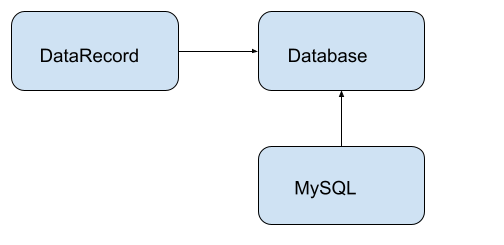
\includegraphics[width=6cm]{dip.png}
   
   We fix this by defining an interface, \texttt{Database}, that tells \texttt{DataRecord} what it should expect and
   tells \texttt{MySQL} what it should provide.
\end{frame} 

%----------- slide --------------------------------------------------%
\begin{frame}
  \frametitle{Reference}
  
  \url{https://fi.ort.edu.uy/innovaportal/file/2032/1/design_principles.pdf}
  
\end{frame}

  
\end{document}
